\documentclass{standalone}
\usepackage{tikz}
\usetikzlibrary{patterns}
\usetikzlibrary{positioning}
\usetikzlibrary{patterns, positioning}
\usetikzlibrary{shapes.misc}
\usepackage[outline]{contour}
\contourlength{1.5pt} 
\usepackage[sfdefault]{ClearSans}

\begin{document}
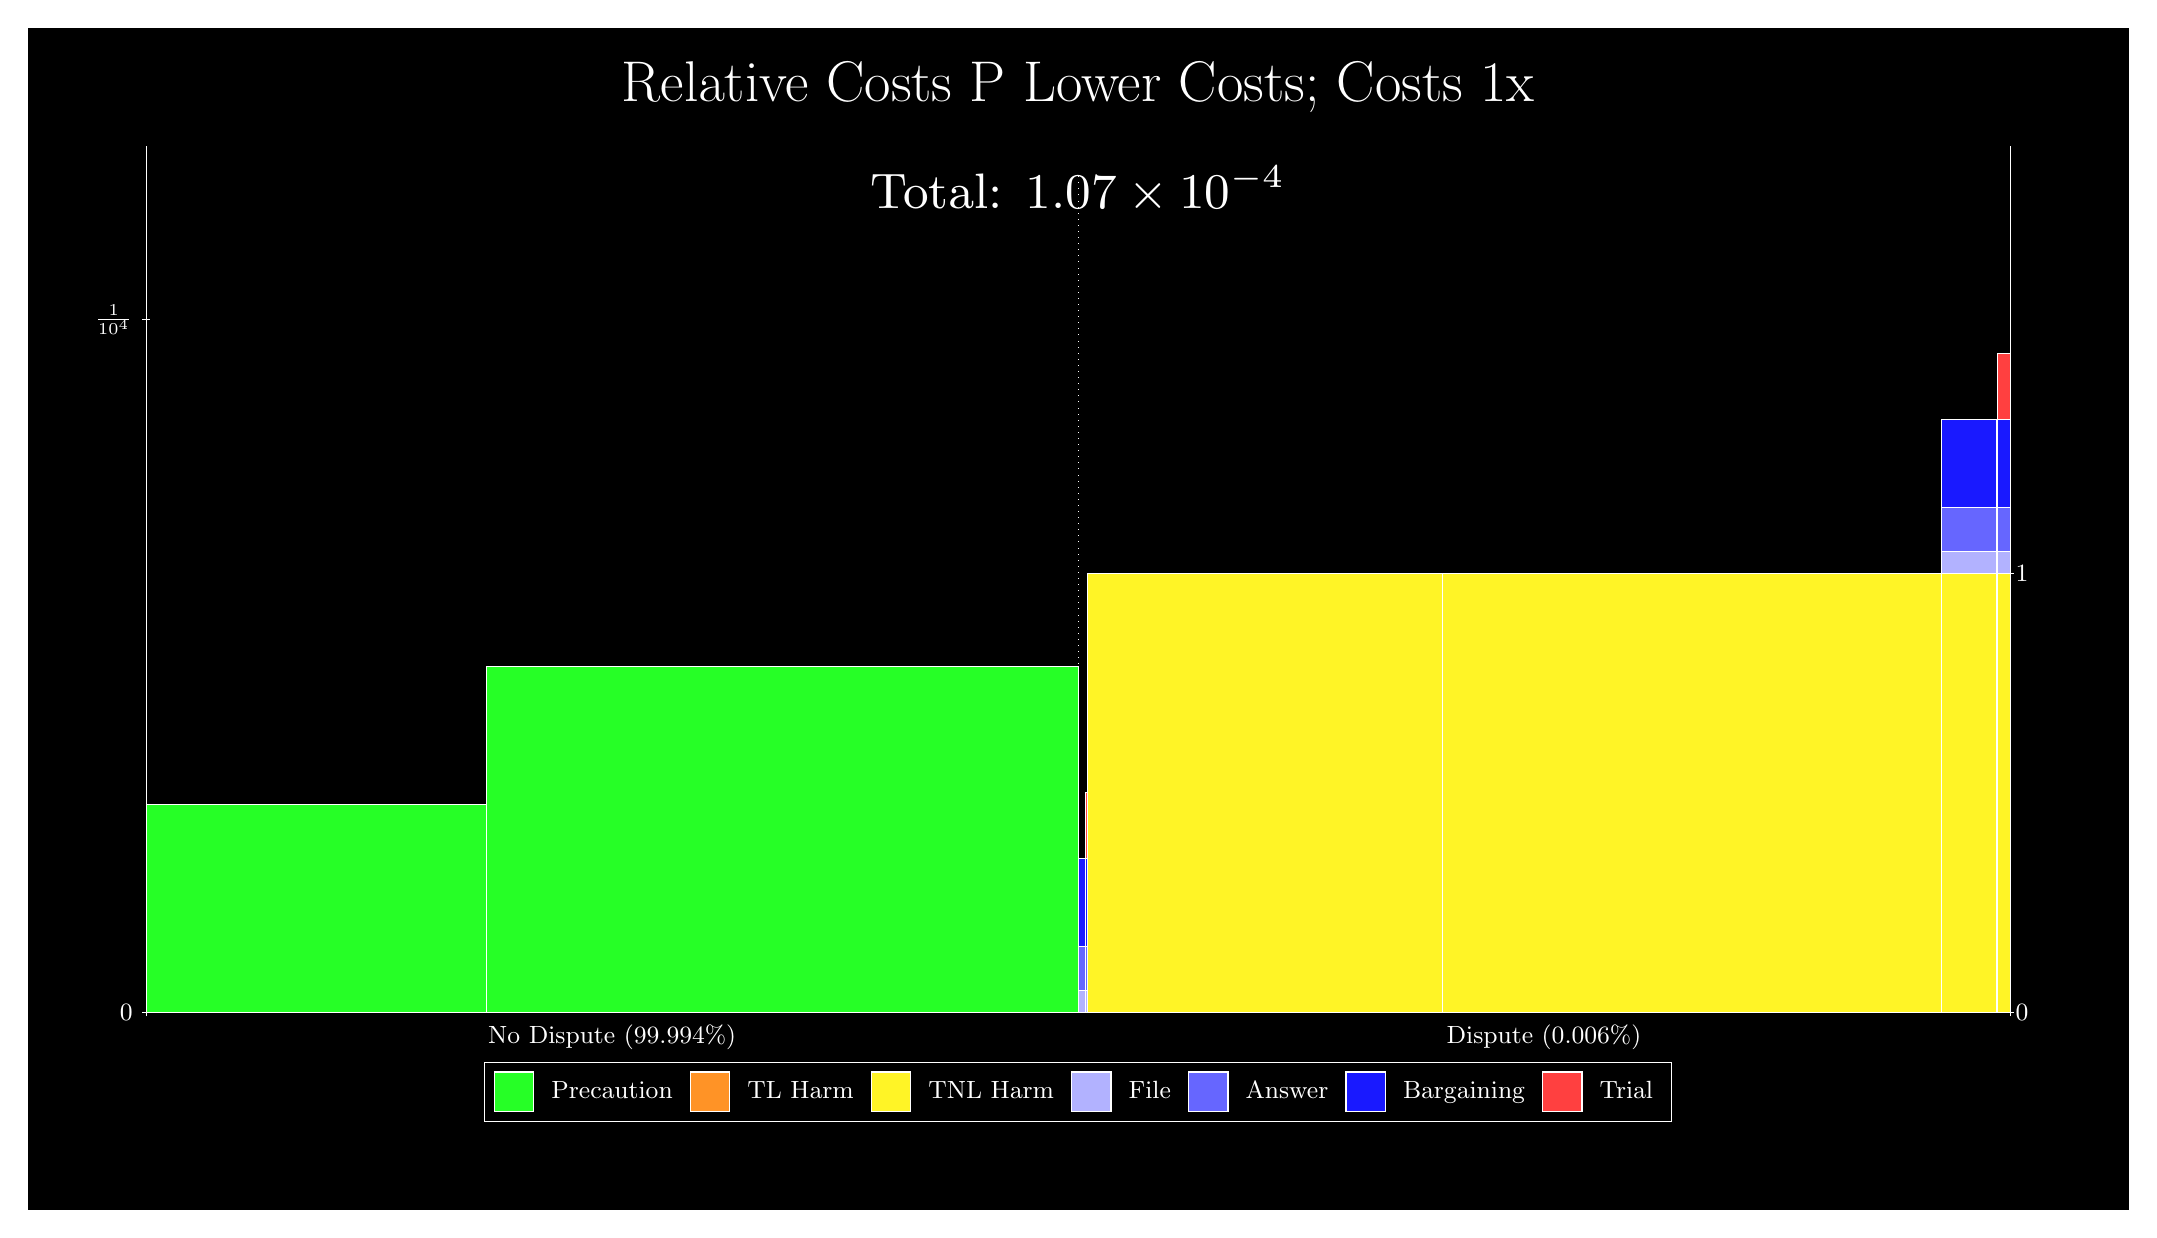
\begin{tikzpicture}
\draw[fill=black] (0,0) rectangle (26.667,15);
\draw[draw=none,text=white] (0,13.5) rectangle (26.667,15) node[midway] {\huge Relative Costs P Lower Costs; Costs 1x};
\draw[fill=green!85,draw=white,very thin] (1.5,2.5) rectangle (5.8205,5.1398);
\draw[fill=green!85,draw=white,very thin] (5.8205,2.5) rectangle (13.333,6.8997);
\draw[fill=green!85,draw=white,very thin] (13.333,2.5) rectangle (13.43,2.5002);
\draw[fill=blue!30,draw=white,very thin] (13.333,2.5002) rectangle (13.43,2.7792);
\draw[fill=blue!60,draw=white,very thin] (13.333,2.7792) rectangle (13.43,3.3372);
\draw[fill=blue!90,draw=white,very thin] (13.333,3.3372) rectangle (13.43,4.4532);
\draw[fill=green!85,draw=white,very thin] (13.43,2.5) rectangle (13.452,2.5002);
\draw[fill=blue!30,draw=white,very thin] (13.43,2.5002) rectangle (13.452,2.7792);
\draw[fill=blue!60,draw=white,very thin] (13.43,2.7792) rectangle (13.452,3.3372);
\draw[fill=blue!90,draw=white,very thin] (13.43,3.3372) rectangle (13.452,4.4532);
\draw[fill=red!75,draw=white,very thin] (13.43,4.4532) rectangle (13.452,5.2902);
\draw[fill=green!85,draw=white,very thin] (13.452,2.5) rectangle (17.959,2.5002);
\draw[fill=yellow!85,draw=white,very thin] (13.452,2.5002) rectangle (17.959,8.0802);
\draw[fill=green!85,draw=white,very thin] (17.959,2.5) rectangle (24.292,2.5003);
\draw[fill=yellow!85,draw=white,very thin] (17.959,2.5003) rectangle (24.292,8.0804);
\draw[fill=green!85,draw=white,very thin] (24.292,2.5) rectangle (25,2.5002);
\draw[fill=yellow!85,draw=white,very thin] (24.292,2.5002) rectangle (25,8.0802);
\draw[fill=blue!30,draw=white,very thin] (24.292,8.0802) rectangle (25,8.3593);
\draw[fill=blue!60,draw=white,very thin] (24.292,8.3593) rectangle (25,8.9173);
\draw[fill=blue!90,draw=white,very thin] (24.292,8.9173) rectangle (25,10.033);
\draw[fill=green!85,draw=white,very thin] (25,2.5) rectangle (25.004,2.5002);
\draw[fill=orange!85,draw=white,very thin] (25,2.5002) rectangle (25.004,8.0802);
\draw[fill=blue!30,draw=white,very thin] (25,8.0802) rectangle (25.004,8.3593);
\draw[fill=blue!60,draw=white,very thin] (25,8.3593) rectangle (25.004,8.9173);
\draw[fill=blue!90,draw=white,very thin] (25,8.9173) rectangle (25.004,10.033);
\draw[fill=green!85,draw=white,very thin] (25.004,2.5) rectangle (25.167,2.5002);
\draw[fill=yellow!85,draw=white,very thin] (25.004,2.5002) rectangle (25.167,8.0802);
\draw[fill=blue!30,draw=white,very thin] (25.004,8.0802) rectangle (25.167,8.3593);
\draw[fill=blue!60,draw=white,very thin] (25.004,8.3593) rectangle (25.167,8.9173);
\draw[fill=blue!90,draw=white,very thin] (25.004,8.9173) rectangle (25.167,10.033);
\draw[fill=red!75,draw=white,very thin] (25.004,10.033) rectangle (25.167,10.87);
\node[font=\small,text=white,anchor=north,scale=2] at (13.333, 13.5) {Total: $1.07\times 10^{-4}$};
\draw[white,very thin] (1.5,2.5) -- (1.5,13.5);
\draw[white,very thin] (1.45,2.5) -- (1.55,2.5);
\node[font=\small,text=white, anchor=east] at (1.45, 2.5) {0};
\draw[white,very thin] (1.45,11.299) -- (1.55,11.299);
\node[font=\small,text=white, anchor=east] at (1.45, 11.299) {$\frac{1}{10^{4}}$};

\draw[white,dotted,very thin] (13.333,2.83) -- (13.333,13.17);
\draw[white,very thin] (25.167,2.5) -- (25.167,13.5);
\draw[white,very thin] (25.117,2.5) -- (25.217,2.5);
\node[font=\small,text=white, anchor=west] at (25.117, 2.5) {0};
\draw[white,very thin] (25.117,8.0801) -- (25.217,8.0801);
\node[font=\small,text=white, anchor=west] at (25.117, 8.0801) {1};

\draw[white,very thin] (1.5,2.5) -- (25.167,2.5);
\draw[white,very thin] (1.5,2.45) -- (1.5,2.55);
\node[font=\small,text=white, anchor=north] at (1.5, 2.45) {};
\draw[white,very thin] (25.167,2.45) -- (25.167,2.55);
\node[font=\small,text=white, anchor=north] at (25.167, 2.45) {};

\node[font=\small,text=white,anchor=south] at (7.4167, 1.9) {No\ Dispute\ (99.994\%)};
\node[font=\small,text=white,anchor=south] at (19.25, 1.9) {Dispute\ (0.006\%)};
\draw (13.3333,2.5) node (B) {};
\begin{scope}[align=center]
\matrix[scale=0.5,draw=white,below=0.5cm of B,nodes={draw},column sep=0.1cm]{
\node[rectangle,draw,minimum width=0.5cm,minimum height=0.5cm,fill=green!85]{}; & \node[draw=none,font=\small,text=white]{Precaution}; &
\node[rectangle,draw,minimum width=0.5cm,minimum height=0.5cm,fill=orange!85]{}; & \node[draw=none,font=\small,text=white]{TL Harm}; &
\node[rectangle,draw,minimum width=0.5cm,minimum height=0.5cm,fill=yellow!85]{}; & \node[draw=none,font=\small,text=white]{TNL Harm}; &
\node[rectangle,draw,minimum width=0.5cm,minimum height=0.5cm,fill=blue!30]{}; & \node[draw=none,font=\small,text=white]{File}; &
\node[rectangle,draw,minimum width=0.5cm,minimum height=0.5cm,fill=blue!60]{}; & \node[draw=none,font=\small,text=white]{Answer}; &
\node[rectangle,draw,minimum width=0.5cm,minimum height=0.5cm,fill=blue!90]{}; & \node[draw=none,font=\small,text=white]{Bargaining}; &
\node[rectangle,draw,minimum width=0.5cm,minimum height=0.5cm,fill=red!75]{}; & \node[draw=none,font=\small,text=white]{Trial}; \\\\
};\end{scope}

\end{tikzpicture}
\end{document}